% Copyright 2018-2019 Melvin Eloy Irizarry-Gelpí
\setcounter{chapter}{5}
\chapter{Kinetic and Elastic Energy}
%
In this experiment you will check that kinetic energy depends on speed in a quadratic way.
%
\section{Preliminary}
%
Energy is a fundamental concept in physics. Unlike force, which is a vector quantity, energy has no intrinsic direction. The \textbf{SI unit} for energy is the joule (J). One joule of energy is equivalent to 1 newton-meter:
\begin{equation}
    1 \text{ J} = 1 \text{ N m}
\end{equation}
There are many forms of energy. \textbf{Kinetic energy} is the energy associated to being in a state of \textbf{motion}. Not surprisingly, the amount of kinetic energy $K$ of an object depends on the amount of mass $m$ and the amount of speed $v$ (not velocity $\vec{v}$). As you will check, the amount of kinetic energy is quadratic in speed:
\begin{equation}
    K = \frac{1}{2} m v^{2}
\end{equation}
Note that kinetic energy cannot be negative, because mass and square speed are always non-negative. If the speed is zero, then you have zero kinetic energy. That is, an object at rest has zero amount of kinetic energy.

A simple direct experiment to test that kinetic energy depends on speed as stated above would involve measuring the speed $v$ and the energy $K$ of a moving object, and checking that the chart with speed and kinetic energy is quadratic. However, we do not have a sensor that measures kinetic energy directly.

When you compress or stretch a spring, you are storing a form of energy known as \textbf{elastic energy}. The amount of elastic energy $U$ stored in a spring with spring constant $k$ and compressed/stretched a distance from equilibrium $x$ is given by
\begin{equation}
    U = \frac{1}{2} k x^{2}
\end{equation}
Note that, like kinetic energy, elastic energy cannot be negative, since $k$ and $x^{2}$ are non-negative. If the distance from equilibrium is zero, then you have zero elastic energy. That is, when the spring is in its relaxed shape, it stores zero amount of elastic energy. The mathematical form of $U$ is very similar to the mathematical form of $K$.

Elastic energy is an example of energy that can be stored over time and used later. Such kinds of energy are known as potential energy. Another important form of energy is \textbf{mechanical energy}, which is just the sum of kinetic energy and any form of potential energy available. The symbol for mechanical energy is $E$.
%
\section{Experiment}
%
You have a cart with a picket fence. The cart can move along a flat track. You can use a photogate to measure the speed of the cart at a given point along the track. You have a spring loop attached to one end of the track. When you push the cart against the spring loop, you compress the spring loop, and you do \textbf{work} (another form of energy). This work is stored on the spring as elastic potential energy. While holding the cart against the spring, the cart is not moving, so the speed of the cart is zero. Thus, at this point in time, the cart has zero kinetic energy. As stated above, the amount of elastic energy depends on how much the spring is compressed. At this point in time the mechanical energy, the sum of the kinetic and elastic energy, is just purely elastic:
\begin{equation}
    E_{1} = K + U = \frac{1}{2} m v^{2} + \frac{1}{2} k x^{2} = \frac{1}{2} k x^{2}
\end{equation}
Then you release the cart. The spring now expands to its equilibrium shape ($x = 0$). As the spring expands, it pushes the cart forward, transferring the elastic energy to the cart. The cart is now moving, so it has kinetic energy. This energy came from the elastic energy of the spring. At this moment, the mechanical energy is just purely kinetic:
\begin{equation}
    E_{2} = K + U = \frac{1}{2} m v^{2} + \frac{1}{2} k x^{2} = \frac{1}{2} m v^{2}
\end{equation}
One of the most important properties of energy is that it is \textbf{conserved}. Specifically, energy cannot be created from nothing, or destroyed into nothing: you can only convert one form of energy into another. Furthermore, in some cases, like this experiment with the cart and the spring loop, the amount of mechanical energy does not change with time. That means that the value of the mechanical energy when the spring is compressed and there is no motion, $E_{1}$, should be equal to the value of the mechanical energy when the spring is not compressed and there is motion, $E_{2}$. That is,
\begin{equation}
    E_{1} = E_{2}
\end{equation}
This means that
\begin{equation}
    \frac{1}{2} m v^{2} = \frac{1}{2} k x^{2}
\end{equation}
Simplifying a bit, you get a relation between the square of speed, and the square of the distance from equilibrium:
\begin{equation}
    v^{2} = \left( \frac{k}{m} \right) x^{2}
\end{equation}
You can experimentally check this relation by measuring the speed of a cart just after being launched by a spring from a certain amount of distance from equilibrium.

For future reference, you can introduce the following quantity
\begin{equation}
    \omega^{2} = \frac{k}{m}
\end{equation}
Here $\omega$, the lowercase Greek letter omega, is known as the \textbf{angular frequency}. The SI unit for angular frequency is radian per second. A radian is a way of measuring the size of an angle. For practical purposes, a radian unit is equivalent to a plain number with no units. In terms of $\omega$, the above relation between $v^{2}$ and $x^{2}$ is given by
\begin{equation}
    v^{2} = \omega^{2} x^{2}
\end{equation}
Thus, a chart with $v^{2}$ in the vertical axis, and $x^{2}$ in the horizontal axis should have a linear shape with slope being close to $\omega^{2}$.
%
\section{Analysis}
%
Here are the steps to follow:
%
\subsection{Measure the position of the equilibrium shape}
%
You can use the marking on the track to measure the position of the cart when the cart is just touching the spring loop and the spring loop is not compressed. This position will be called $d_{0}$ and will be used next to find the distance from equilibrium.
%
\subsection{Calculate the distance from equilibrium}
%
You recorded the launch position $d$ of the cart. Together with the equilibrium position $d_{0}$, you can calculate the distance from equilibrium $x$:
\begin{equation}
    x = d_{0} - d
\end{equation}
This definition of $x$ guarantees that $x$ will be positive.
%
\subsection{Find the 3-run average speed}
%
It is good practice to, for a given launch position, repeat a launch and record at least three consistent values of the speed of the cart. You can find the 3-run average speed and use that as your best estimate for the speed of the cart when being launched from that particular position.
%
\subsection{Visualize velocity versus distance}
%
You can make a chart with speed $v$ in the vertical axis and distance from equilibrium $x$ in the horizontal axis. According to the expected model, the chart should have a linear shape and the slope should be related to $\omega$. However, since you do not know the value of the spring constant $k$, you cannot determine the expected value of $\omega$. Indeed, you can use this experiment to measure $\omega$.

In my case, Figure \ref{figure:06.v} shows the relation between $v$ and $x$. As you can see, the relation is linear. The chart includes the best-fit line.
%
\subsection{Visualize squared velocity versus squared distance}
%
The relation between $v$ and $x$ from energy conservation involves the square quantities. It does not hurt to check the linear quantities, but a real test should involve the squares. In new spreadsheet columns you can calculate the square speed and the square of the distance from equilibrium. Then you can make a chart with $v^{2}$ in the vertical axis and $x^{2}$ in the horizontal axis. The expectation is that this chart should also have a linear shape, with a very small intercept, and a slope related to $\omega^{2}$.

In my case, Figure \ref{figure:06.v.2} shows the relation between $v^{2}$ and $x^{2}$. The data also has a linear shape.
%
\subsection{Estimate the value of the spring constant}
%
You can use a digital scale to find the value of the mass of the cart, and the mass of the picket fence. The sum of these masses, gives you the total mass of the object that the spring pushes away. In Table \ref{table:06.mass} you can find the values for my case.

The slope in Figure \ref{figure:06.v.2} provides an estimate for $\omega^{2}$:
\begin{equation}
    \omega^{2} \approx 62.3 \text{ rad}^{2}\text{/s}^{2}
\end{equation}
Using the definition of $\omega^{2}$ to solve for $k$ gives
\begin{equation}
    k = \omega^{2} m \approx \left( 62.3 \text{ rad}^{2}\text{/s}^{2} \right) \left( 0.5218 \text{ kg} \right) = 31.508 \text{ N/m}
\end{equation}
The spring constant for the spring loop will be slightly different for each spring, but your result should be close to 30 N/m.
%
\section{My Data}
%
My raw data for launch position and speed is in Table \ref{table:06.data}. The first column has the position of launch. The second column has the corresponding distance from equilibrium. The third, fourth, and fifth columns have the speed of the cart measured by the photogate. The last column has the 3-run average speed. I considered seven compressed distances, plus the first row that corresponds to an uncompressed spring.
%
\section{Your Data}
%
Your data should be very similar to mine, but the actual launch positions might be different due to the varying shapes of the spring loops. You should have a total of eight data points.
%
\newpage
\section{Your Laboratory Report}
%
Your lab report should include the following:
\begin{enumerate}
    \item A table like Table \ref{table:06.mass} with the mass values you measured.
    \item A table like Table \ref{table:06.data} with the positions you used for launching the cart, the corresponding distance from equilibrium, the speed you measured, and the 3-run average speed.
    \item A chart with $v^{2}$ in the vertical axis, and $x^{2}$ in the horizontal axis. Include the best fit line, along with the equation.
    \item Use the slope value to estimate $\omega^{2}$. Then use this estimate of $\omega^{2}$ and the total mass of the object to estimate the value of the spring constant $k$ for the spring loop.
\end{enumerate}
%
\newpage
\section{Tables}
%
\vspace{\stretch{1}}
\begin{table}[ht]
    \centering
    \begin{tabular}{|l|r|}
        \hline
        Name & Value (kg) \\
        \hline
        Mass of cart & 0.5088 \\
        Mass of picket fence & 0.013 \\
        \hline
        Total mass & 0.5218 \\
        \hline
    \end{tabular}
    \caption{Mass measurements}
    \label{table:06.mass}
\end{table}
\vspace{\stretch{1}}
%
\begin{table}[ht]
    \centering
    \begin{tabular}{|l|r|r|r|r|r|}
        \hline
        $d$ (cm) & $x$ (cm) & $v_{1}$ (m/s) & $v_{2}$ (m/s) & $v_{3}$ (m/s) & Average $v$ (m/s) \\
        \hline
        11 & 0 & 0 & 0 & 0 & 0 \\
        10 & 1 & 0.079 & 0.081 & 0.077 & 0.079 \\
        9.5 & 1.5 & 0.122 & 0.124 & 0.125 & 0.124 \\
        9 & 2 & 0.162 & 0.164 & 0.151 & 0.159 \\
        8.5 & 2.5 & 0.197 & 0.211 & 0.199 & 0.202 \\
        8 & 3 & 0.236 & 0.235 & 0.238 & 0.236 \\
        7.5 & 3.5 & 0.274 & 0.274 & 0.279 & 0.276 \\
        7 & 4 & 0.317 & 0.312 & 0.322 & 0.317 \\
        \hline
    \end{tabular}
    \caption{Raw Data}
    \label{table:06.data}
\end{table}
\vspace{\stretch{1}}
%
\newpage
\section{Figures}
%
\vspace{\stretch{1}}
\begin{figure}[ht]
    \centering
    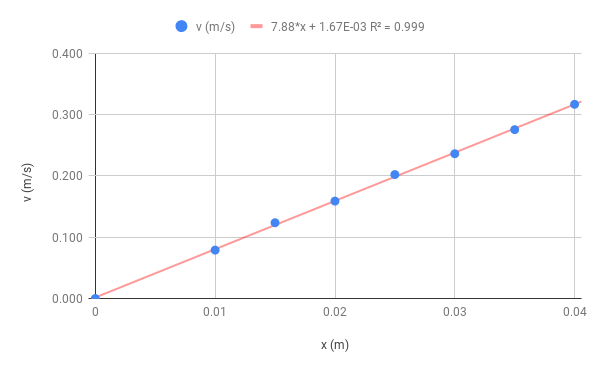
\includegraphics[scale=0.71]{image/06-kinetic/v.png}
    \caption{Velocity versus distance from equilibrium}
    \label{figure:06.v}
\end{figure}
\vspace{\stretch{1}}
%
\begin{figure}[ht]
    \centering
    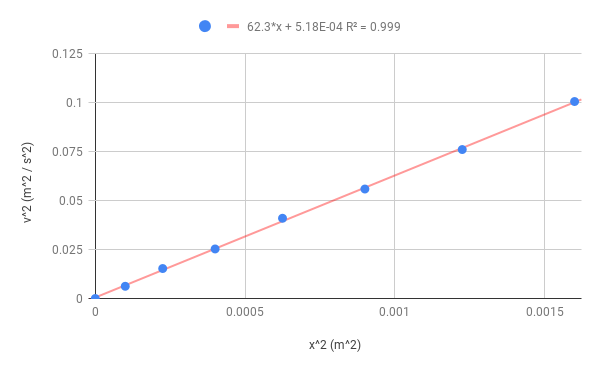
\includegraphics[scale=0.71]{image/06-kinetic/v2.png}
    \caption{Square of Velocity versus square of distance from equilibrium}
    \label{figure:06.v.2}
\end{figure}
%